\section{Ablation}\label{sec:ablation}

\subsection{Components of the refinement}

The ablation removes one component of the refinement at a time on the lattice task and the seeds of the main result. All variants share the start, the budget and the scoring, and the variant with the default components reproduces the module of the engine to a difference of \ablBCheck{} on the spread for every seed, and the variant with the weight update on reproduces the module with that option to \ablBWeightsCheck{}, so the rows are the module with components removed or added. Table~\ref{tab:ablb1} gives the crosstalk device and Table~\ref{tab:ablb1full} the full device; Fig.~\ref{fig:ablation} shows the per-seed spreads. The statistics are the median and the
range of the spread, the geometric-mean factor over the reference of Eq.~\ref{eq:factor} with its 95 percent interval, and the median efficiency ratio, for \ablBN{} seeds on the crosstalk device and \ablBFN{} on the full device.

\begin{table}[t]
\centering\small
\caption{Ablation of the refinement on the crosstalk device, $10\times10$ lattice task, \ablBN{} seeds. Each row removes one component, adds the weight update or changes one parameter; $\sigma$ is the relative standard deviation on the device, the factor is the geometric mean over the better of the two phase-fixed baseline runs with its 95 percent interval, and the last column is the median ratio of the efficiencies.}
\label{tab:ablb1}
\resizebox{\textwidth}{!}{\begin{tabular}{@{}l r r r r@{}}
\toprule
Variant & $\sigma$ median (\%) & $\sigma$ range (\%) & Factor over phase-fixed WGS, 95\% interval & $e$ ratio \\
\midrule
device-aware refinement, default (no weight update) & 0.030 & 0.016 to 0.032 & 201.3 (132.9 to 304.9) & 0.999 \\
with the weight update (the 0.02.003 form) & 0.205 & 0.157 to 0.298 & 24.4 (17.5 to 34.1) & 0.995 \\
without the device-aware phase step & 6.508 & 4.861 to 7.418 & 0.8 (0.7 to 1.0) & 1.000 \\
without the best-iterate safeguard & 0.030 & 0.016 to 0.032 & 201.3 (132.9 to 304.9) & 0.999 \\
device model removed from the loop & 5.153 & 4.721 to 5.445 & 1.0 (1.0 to 1.0) & 1.000 \\
1 conjugate-gradient step per iteration & 0.469 & 0.262 to 0.591 & 12.3 (8.1 to 18.7) & 1.000 \\
6 conjugate-gradient steps per iteration & 0.028 & 0.004 to 0.072 & 218.2 (47.9 to 994.8) & 0.999 \\
warm start only (no iteration) & 6.508 & 4.861 to 7.418 & 0.8 (0.7 to 1.0) & 1.000 \\
\bottomrule
\end{tabular}
}
\end{table}

\begin{table}[t]
\centering\small
\caption{Ablation of the refinement on the full device ($\parBits$-bit phase, crosstalk, fill factor \parFill{}), \ablBFN{} seeds, same task and statistics as Table~\ref{tab:ablb1} for the components that matter; the intervals use only five seeds and are wide.}
\label{tab:ablb1full}
\resizebox{\textwidth}{!}{\begin{tabular}{@{}l r r r r@{}}
\toprule
Variant & $\sigma$ median (\%) & $\sigma$ range (\%) & Factor over phase-fixed WGS, 95\% interval & $e$ ratio \\
\midrule
device-aware refinement, default (no weight update) & 0.242 & 0.202 to 0.335 & 23.5 (18.6 to 29.6) & 0.997 \\
with the weight update (the 0.02.003 form) & 0.729 & 0.597 to 1.163 & 7.4 (5.7 to 9.8) & 0.990 \\
without the device-aware phase step & 6.866 & 5.115 to 8.320 & 0.8 (0.7 to 1.0) & 0.999 \\
without the best-iterate safeguard & 0.242 & 0.202 to 0.335 & 23.5 (18.6 to 29.6) & 0.997 \\
device model removed from the loop & 5.786 & 5.171 to 5.969 & 1.0 (1.0 to 1.0) & 1.000 \\
warm start only (no iteration) & 6.866 & 5.115 to 8.320 & 0.8 (0.7 to 1.0) & 0.999 \\
\bottomrule
\end{tabular}
}
\end{table}

\begin{figure}[t]
\centering
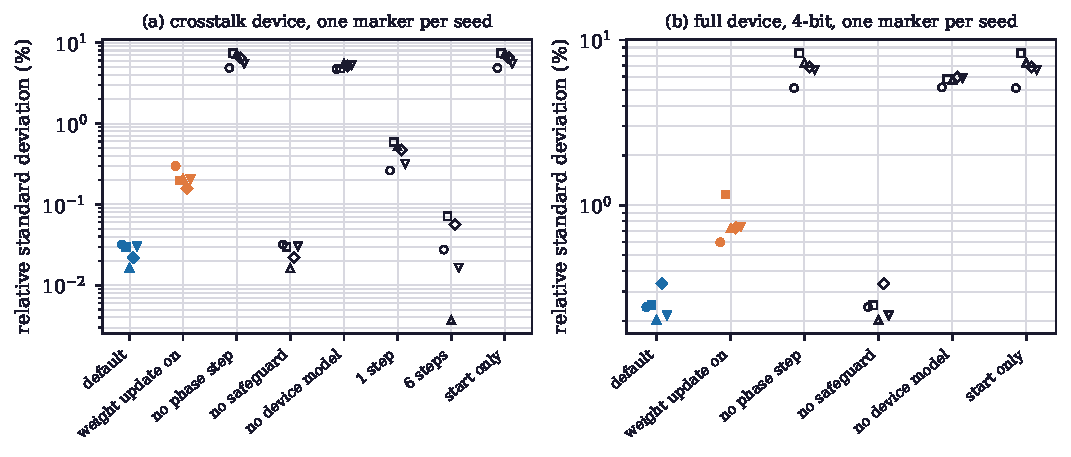
\includegraphics[width=\textwidth]{fig-ablation.pdf}
\caption{Ablation per seed. (a) Relative standard deviation on the crosstalk device of the variants of the refinement (logarithmic axis). (b) The same variants on the full device. Filled blue markers are the default refinement, filled orange markers the variant with the weight update; one marker per seed.}
\label{fig:ablation}
\end{figure}

The device model in the loop and the conjugate-gradient step carry the gain. With the device model removed from the loop the spread returns to the level of the baseline, \ablBNoModelSig{} percent, \ablBModelRatio{} times above the default \ablBFullSig{} percent, and on the full device \ablBFNoModelSig{} against \ablBFFullSig{} percent, \ablBFModelRatio{} times. Without the conjugate-gradient step the variant has no way to improve on its start: with the weights at one, the projection of weighted GS read on the device returns the warm start seed by seed (the rows of the two variants are identical), because the safeguard picks the start when no iterate of the projection has a lower spread. Its median is \ablBNoStepSig{} percent, a factor of \ablBNoStepFac{} (interval \ablBNoStepFacLo{} to \ablBNoStepFacHi{}) over the baseline, \ablBStepRatio{} times above the default. The warm start alone leaves \ablBWarmSig{} percent, so the conjugate-gradient iterations on the device, not the start, produce the result. The number of steps matters less than their presence: one step per outer iteration leaves \ablBStepsOneSig{} percent (factor \ablBStepsOneFac{}), and six steps reach \ablBStepsSixSig{} percent with a wider interval (\ablBStepsSixFacLo{} to \ablBStepsSixFacHi{}) than three, which is not better on the median.

The weight update does not help, it hurts. With the update on, the median spread is \ablBWeightsSig{} percent (range \ablBWeightsSigMin{} to \ablBWeightsSigMax{}), \ablBWeightsRatio{} times higher than the \ablBFullSig{} percent of the default (range \ablBFullSigMin{} to \ablBFullSigMax{}), at an efficiency ratio of \ablBWeightsEff{} against \ablBFullEff{}; the geometric-mean factor over the baseline falls from \ablBFullFac{} (interval \ablBFullFacLo{} to \ablBFullFacHi{}) to \ablBWeightsFac{} (interval \ablBWeightsFacLo{} to \ablBWeightsFacHi{}). On the full device the
spread with the update is \ablBFWeightsSig{} percent against \ablBFFullSig{} percent without it, \ablBFWeightsRatio{} times higher. H6 holds on both devices: the integral action of the weights, which the earlier design of the method gave as its reason, is not needed when three conjugate-gradient steps follow the target on this task, and it costs spread. This is in line with Conjecture~\ref{conj:windup}; the conjecture itself, that the weights wind up, is compatible with these data and is not proved by them. The safeguard did not act on these seeds: with and without it the spreads are identical (\ablBNoGuardSig{} percent, the same on the full device), as Proposition~\ref{prop:guard} allows, since the last iterate is the best admissible one on both devices. Its value is on the geometries of the benchmark where the last iterate would lose too much light, and on a run that winds up with the update on.

\subsection{The weight update and the loss on the lattices of the benchmark}

The same comparison on the lattices of the benchmark answers whether the result of the acceptance task carries to other geometries and whether the loss matters there. Each cell is the benchmark's own record, run through the engine's runner and scored against the C08 device ($4$-bit phase, crosstalk, fill factor and flicker) at \geoIters{} outer iterations for \geoSeeds{} seeds, with the weight update and the loss switched by the module's options (Table~\ref{tab:ablb1geo}, Fig.~\ref{fig:geo}). On the ideal model all three forms reach a spread of at most \geoAIdealMax{} percent on the square lattice and \geoBIdealMax{} percent on the others. On the device the outcome depends on the geometry. On the square lattice the default halves the spread of the variant with the weight update, \geoANSig{} against \geoAWSig{} percent, with the lower spread on \geoALower{} of \geoASeeds{} seeds, at a lower efficiency, \geoANEff{} against \geoAWEff{}; the normalized-error loss gives \geoASSig{} percent, with the default lower on \geoALowerSchroff{} of \geoASeeds{} seeds. On the ring of 36 traps the weight update is better, \geoBWSig{} against \geoBNSig{} percent, with the default lower on \geoBLower{} seed of \geoBSeeds{}, and the normalized-error loss gives \geoBSSig{} percent (the default lower on \geoBLowerSchroff{} seeds). On the random set the three differ by a few percent of the spread (\geoCWSig{}, \geoCNSig{} and \geoCSSig{} percent), the default being lower than the weight update on \geoCLower{} seeds and than the normalized-error loss on \geoCLowerSchroff{}. On the quasi-periodic set the three medians are the same, \geoDWSig{} percent; the variants return the same spread on \geoDSameSeeds{} of the \geoDSeeds{} seeds, and on the others they differ (Fig.~\ref{fig:geo}). That is the measurement; the data do not say why the variants coincide on those seeds, and no explanation is offered.

\begin{table}[t]
\centering\small
\caption{The refinement with the weight update, by default and with the normalized-error loss of Schroff et al.\ on the lattices of the benchmark, C08 device, \geoIters{} outer iterations: median over \geoSeeds{} seeds of the relative standard deviation $\sigma$ and of the efficiency $e$ on the device, and the number of seeds on which the default has the lower spread than the weight update and than the normalized-error loss.}
\label{tab:ablb1geo}
\resizebox{\textwidth}{!}{\begin{tabular}{@{}l r r r r r r r r@{}}
\toprule
Geometry & $\sigma$ with weights (\%) & $\sigma$ default (\%) & $\sigma$ Schroff (\%) & $e$ with & $e$ default & $e$ Schroff & seeds default below weights & seeds default below Schroff\\
\midrule
G1, Square 10 x 10 & 27.14 & 13.64 & 14.03 & 0.598 & 0.563 & 0.566 & 5 of 5 & 4 of 5\\
G2, Ring of 36 traps & 8.03 & 8.46 & 8.55 & 0.453 & 0.462 & 0.461 & 1 of 5 & 3 of 5\\
G3, Random 100 traps & 4.43 & 4.27 & 4.14 & 0.402 & 0.409 & 0.408 & 4 of 5 & 1 of 5\\
G4, Quasi-periodic 119 & 86.01 & 86.01 & 86.01 & 0.504 & 0.504 & 0.504 & 1 of 5 & 1 of 5\\
\bottomrule
\end{tabular}
}
\end{table}

\begin{figure}[t]
\centering
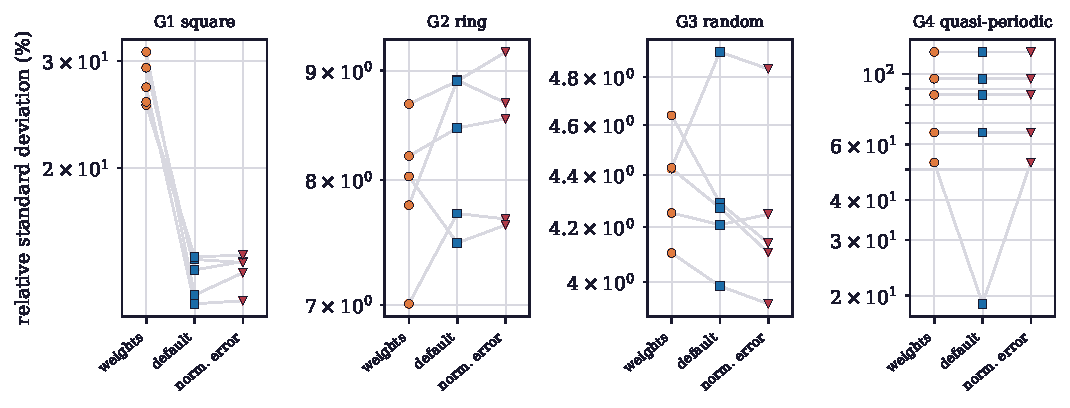
\includegraphics[width=\textwidth]{fig-geo.pdf}
\caption{Spread on the device per seed of the three forms of the refinement on the four lattices of the benchmark, \geoIters{} outer iterations. Each panel is one geometry; markers of the same seed are joined; the vertical axes are logarithmic.}
\label{fig:geo}
\end{figure}

Neither the weight update nor the loss dominates on these lattices. The default has the lower median spread than the weight update on the square lattice and the random set and the higher on the ring, and its median spread is within a few percent of that of the normalized-error loss on all four lattices; on the square lattice the difference between the default and the normalized-error loss is smaller than the difference between seeds. The benchmark's table at \benchOneBudget{} iterations is the phase-fixed reference for the same lattices (Table~\ref{tab:bench}); Table~\ref{tab:ablb1geo} has no phase-fixed run at the budget of \geoIters{} outer iterations, so the two tables are read side by side and not subtracted.
